\documentclass[12pt]{article}
\usepackage[hmargin={1in},vmargin={1in,1in},foot={.6in}]{geometry}   
\geometry{letterpaper}              
\usepackage{color,graphicx}
\usepackage{setspace}
\usepackage{amsmath}
\usepackage{amssymb}
\usepackage{varioref}
\usepackage{textcomp}
\usepackage{textcomp}
\usepackage{mflogo}
\usepackage{wasysym}
\usepackage[normalem]{ulem}
\usepackage{hyperref}

\newcommand{\HRule}{\rule{\linewidth}{0.25mm}}

\usepackage{fancyhdr} % This should be set AFTER setting up the page geometry
\pagestyle{plain} % options: empty , plain , fancy
\lhead{}\chead{}\rhead{}
\renewcommand{\headrulewidth}{.5pt}
\lfoot{}\cfoot{\thepage}\rfoot{}
\newcommand{\txtp}{\textipa}
\renewcommand{\rm}{\textrm}
\newcommand{\sem}[1]{\mbox{$[\![$#1$]\!]$}}
\newcommand{\lam}{$\lambda$}
\newcommand{\lan}{$\langle$}
\newcommand{\ran}{$\rangle$}
\newcommand{\type}[1]{\ensuremath{\left \langle #1 \right \rangle }}

\newcommand{\bex}{\begin{exe}}
\newcommand{\eex}{\end{exe}}
\newcommand{\bit}{\begin{itemize}}
\newcommand{\eit}{\end{itemize}}
\newcommand{\ben}{\begin{enumerate}}
\newcommand{\een}{\end{enumerate}}

\newcommand{\gcs}[1]{\textcolor{blue}{[gcs: #1]}}
\definecolor{Green}{RGB}{10,200,100}
\newcommand{\ndg}[1]{\textcolor{Green}{[ndg: #1]}}
\newcommand{\jd}[1]{\textcolor{red}{[jd: #1]}}

\thispagestyle{plain}

\begin{document}

{\flushright

\vspace{25pt}
Gregory Scontras\\
Noah D.~Goodman\\
Department of Psychology\\
Stanford University\\
Stanford, CA 94305\\[20pt]

\noindent June XXX, 2016\\[20pt]}


\noindent Dear Editor,\\

\noindent We would like to thank you and the three anonymous reviewers for your helpful comments on our paper, ``Subjectivity predicts adjective ordering preferences.'' As you will recall, you highlighted the following concerns: 

\ben

\item \emph{Reviewer 2 questioned whether endorsements of `together' paraphrases are indicative of collective interpretations.}

\item \emph{Reviewer 2 raised alternative accounts of the contextual effects on the interpretation of bare sentences.}

\item \emph{Reviewer 2 raised the possibility of `cumulative' construals in the interpretation of bare sentences.}

\item \emph{Reviewer 2 mentioned prior published research that is relevant for Experiment 1.}

\item \emph{Reviewer 2 recommends highlighting the novel contribution of the speaker's epistemic state.}

\item \emph{Reviewer 1 was concerned that the effects of contextual predictability were only tested on a limited set of words and contexts.}

We followed the reviewer's suggestion and ran an additional experiment (\emph{Expt.~4: Generalizing our findings}), which tests the predictions of contextual predictability and speaker knowledge with a much larger set of 25 dimensional adjectives (cf.~our original set of three). The new results replicate our original findings and add nuance to our account, highlighting an additional aspect of the pragmatic calculus of utterance disambiguation: the probability that a specific interpretation would truthfully describe a state of affairs. We expand on this point in our response to Reviewer 1's point 1 below.

\item \emph{Reviewer 1 requested more information about the ratings data to get a better sense of individual response patterns.}

We have replaced most of our bar plots with the more informative violin plots that Reviewer 1 suggested. We expand on this point in our response to Reviewer 1's point 2 below.

\item \emph{Reviewer 3 raised an alternative account of subjects' interpretation of `tall' in regular vs. irregular contexts.}

The reviewer raised the issue of how the likely truth of a given interpretation might affect its probability: interpretations that are more obviously true should be more probable. We explore this idea in our new experiment (\emph{Expt.~4: Generalizing our findings}; cf.~our response to the Editor's point 6 above), and find that an interpretation's probability of being judged true affects that interpretation's overall probability. We expand on this point below in our responses to Reviewer 1's point 1 and Reviewer 3's point 3.

\een


\noindent In the remainder of this letter, we consider in more detail each of the reviewers' concerns.


\newpage

\subsubsection*{Reviewer 1:}

\ben

\item \emph{My largest reservation is that the main result, which is that contextual predictability affects whether an interpretation is distributive or collective, is really only experimentally evaluated (in Experiment 3) for three words (\emph{big}, \emph{heavy}, and \emph{tall}) in one context (moving boxes). The paper would be much stronger if either the number of words were broader, or the contexts were broader.}

We have followed the reviewer's suggestion, investigating contextual predictability and speaker knowledge with a much broader set of predicates (\emph{Expt.~4: Generalizing our findings}). We extended the Cubert paraphrase endorsement paradigm from Expt.~3, testing a total of 25 dimensional adjectives (cf.~the three predicates tested in Expt.~3). We grouped these adjectives into seven different semantic classes (capacity, depth, height, length, size, weight, and width) and two polarities (positive and negative; e.g., \emph{tall} vs. \emph{short}). The results of the new experiment 1) replicate the results of Expt.~3 with a broader set of lexical items, and 2) add nuance to our claims about contextual predictability. We continue to find that collective interpretations depend on the contextual predictability of collective properties, such that increasing predictability by regularizing arrangements increases rates of collective interpretations. However, to increase predictability one must regularize the specific dimension under discussion (e.g., the height dimension for \emph{tall} but not \emph{long}, or the width dimension for \emph{narrow} but not \emph{deep}). Moreover, we observed that contextual predictability interacts with yet another aspect of the pragmatic calculus that influences interpretation choice, namely the probability that a specific interpretation would truthfully describe a state of affairs. When an interpretation appears unlikely to be true (e.g., describing a tall stack of boxes as collectively short), listeners are unlikely to attribute that interpretation to speakers' utterances. \gcs{add more}

\item \emph{I really liked Experiment 2 but it is possible that these means simply reflect different distributions of extreme values. For this reason I think you should include violin plots as well as means, just to assure ourselves that that isn't happening.}

We have followed this suggestion and replaced all but one of our ratings bar plots with violin plots. The new violin plots include condition means and bootstrapped 95\% confidence intervals. The plots communicate at least as much information as our original bar plots, and have the added benefit of allaying the reviewer's worry that the diverging means reflect different distributions of extreme values. The one plot that we have not replaced with a violin plot appears in Figure 4, which plots mean collective endorsement ratings for each of the 40 unique sentences tested in Expt.~2a. We chose to keep the bar plots because we found the violin plots to be uninformative at such a large scale, and because we now use violin plots in Figure 5, which zooms in on the relevant sentences from Figure 4. Here is what a violin plot of the data in Figure 4 would look like:

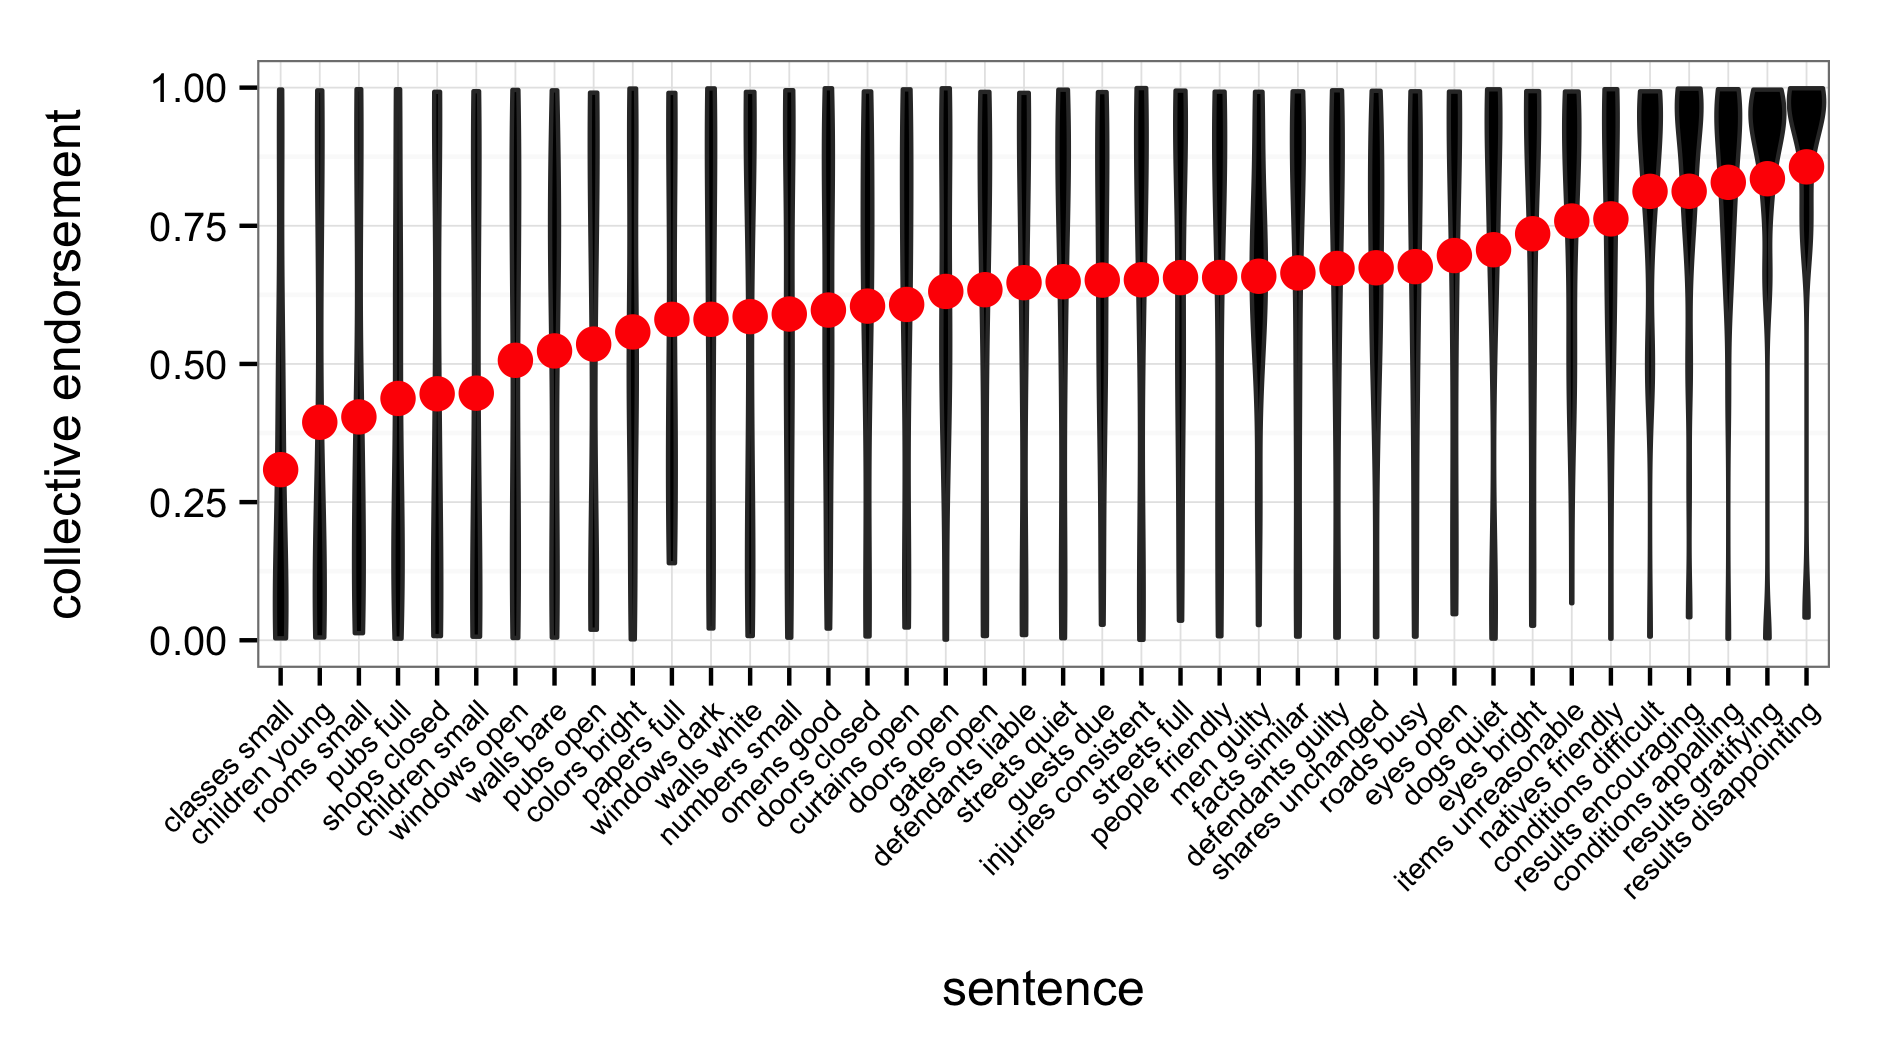
\includegraphics[width=\linewidth]{plots/sentence_plot_violin.eps}

\item \emph{I'm kind of surprised there were only two alternatives considered for the speakers knowledge state: full or sum. It seems to me that the non-regular condition corresponds to a situation that is neither: the speaker has knowledge of the individual boxes, and can kind of vaguely infer what the full set might look like (e.g., by mentally stacking them) but only noisily so.}

\item \emph{There needs to be more information about the experimental participants. Nationality? Age? How much were they paid?}

\een



\subsubsection*{Reviewer 2:}

\ben

\item \emph{The authors should situate their findings against the backdrop of our previous experimental work on \emph{each} and \emph{together}.}

\item \emph{The authors should highlight the role of the speaker's epistemic state.}

\item \emph{The authors set up the contrast between distributive and collective interpretations without mentioning the possibility of cumulative interpretations. This reading should be mentioned.}

\item \emph{The authors repeatedly refer to \emph{together} as though it unambiguously signals a collective interpretation, but this is most definitely not the case! Cite previous experimental work on the flexbility of \emph{together}.}

\item \emph{The authors take participants' willingness to accept the sentence The NOUNS together were ADJECTIVE as compatible with the speaker's intended meaning as an indication of their willingness to allow a collective interpretation of the target sentence. But this is inherently problematic, because that sentence does not unambiguously signal a collective meaning to the participant! Take the following example: ``The boys together were smiling.'' The true `collective' interpretation of this sentence is that each boy contributed in such a way that collectively the boys created what can be truthfully described as a smiling event, and no one boy has this property, while the group does.}

\item \emph{Participants may have been inserting a silent collectivizing noun (e.g., \emph{box}, \emph{pile}, \emph{stack}) into the together sentences.}

\item \emph{A plural definite description like the boxes maps onto an atomic join semi-lattice. There is therefore semantically in the representation, a maximal element (just as there is with the singular definite description the box). It is entirely possible that participants were predicating of this maximal element, which would make it seem as though they are accessing the collective interpretation, when in fact they are not.}

\item \emph{The authors are aware of the context-dependence of the gradable adjectives that are the target of their investigation (e.g., \emph{big}, \emph{tall}, \emph{heavy}), but they do not make too much of this in the paper. One possibility is that \emph{The boxes (together) are big} could be taken to mean something like, `If you look at the boxes all together, then they form a comparison class such that they surpass some relevant threshold and could be considered to be big.'}

\item \emph{Don't predicates such as \emph{have brown eyes} have to apply at the atomic level? If so, then aren't there predicates out there for which young language learners must learn that they obligatorily apply to atomic individuals that are members of a plurality? And if this is the case, then couldn't \emph{big} and \emph{tall} be stubbornly distributive at the lexical level?}

\item \emph{If there are predicates like gather that must apply at the level of the group (i.e., they are stubbornly collective) why is it not unreasonable to think that these predicates contrast with another category, whose denotation requires them to apply at the atomic level, and another category, which are flexible in the level to which they apply?}

\item \emph{I am not able to interpret \emph{These boxes are big} collectively. (I am a native speaker of American English.) I can, however, maybe access a collective interpretation of \emph{These boxes are tall}. This paper doesn't allow me to understand why I am encountering an introspective difference between these two predicates, or why we see one in the experimental results.}

\een


\subsubsection*{Reviewer 3:}

\ben

\item \emph{For experiment 2, I wonder if some of the nouns are really plural (\emph{conditions}, \emph{results}).}

This is a reasonable concern about our corpus-based experimental items, which we selected solely on the basis of frequency of occurrence. We ran the follow-up in Expt.~2a with a more targeted set of items in part to allay this concern. There, subject nouns denoted real-world (as opposed to abstract or psychological) entities.

\item \emph{For experiment 2, some of the collective interpretations imply a distributive one (\emph{the dogs were quiet}).}

\item \emph{In experiment 3's irregular conditions, maybe the participants are thinking: Cubert wouldn't say the boxes were collectively tall unless they were collectively VERY tall; so here he must have been referring to the individual boxes. Admittedly, I'm not sure how this would apply to ``big''. This alternative story suggests that you should control for the actual height of the boxes when predicting responses. Maybe the difference between ``regular'' and ``irregular'' conditions just reflects the difference in total average height in the ``tall'' case.}

The results of our new experiment (\emph{Expt.~4: Generalizing our findings}) explore and support this intuition: the probability that a specific interpretation would truthfully describe a state of affairs enters into the pragmatic calculus of utterance disambiguation. As suspected, interpretations that are more likely to be true (e.g., a collective interpretation for \emph{narrow} with a tall, thin stack of boxes) are more likely. We expand on this finding in our discussion of Expt.~4's results. \gcs{add more depending on whether we include the polarity model}

\een


\newpage

\noindent Thank you again for the thorough and thoughtful comments on our work. We hope that you will like the new version of the paper. Please let us know if you require additional information. We look forward to hearing from you!\\[25pt]


\noindent Yours sincerely,\\[10pt]

\noindent Gregory Scontras and Noah D.~Goodman



\end{document}














